\documentclass[11pt,a4paper]{article}
\usepackage[utf8]{inputenc}
\usepackage[portuguese]{babel}
\usepackage{graphicx}
\usepackage{geometry}
\usepackage{float}
\usepackage{hyperref}
\usepackage{amsmath}
\usepackage{xcolor}
\usepackage{titlesec}
\usepackage{booktabs}

\geometry{margin=2.5cm}

\title{
    \vspace{-1.5cm}
    \textbf{Fundamentos de Inteligência Artificial} \\
    \large Trabalho Prático Nº 2: The evolution of Lunar Lander
}

\author{
    \textbf{[O Seu Nome]} -- \texttt{[Número de Estudante]} -- \texttt{[Email]} \\
    \textbf{[Nome do Colega]} -- \texttt{[Número de Estudante]} -- \texttt{[Email]} \\
    \textbf{[Nome do Colega 3 (se aplicável)]} -- \texttt{[Número]} -- \texttt{[Email]} \\
    Turma Prática: [Sua Turma]
}
\date{Maio de 2026}

\begin{document}

\maketitle

\begin{abstract}
Este relatório descreve o processo de modelação, implementação e otimização de um Algoritmo Evolucionário (Neuroevolução) para controlar uma nave espacial no simulador Lunar Lander. O projeto divide-se em duas metas: a primeira foca-se num ambiente estático e a segunda na introdução de correntes de ar (vento). O documento detalha as escolhas dos operadores genéticos, os estudos paramétricos realizados e a evolução das funções objetivo ("Reward Shaping") que permitiram à rede neuronal aprender a aterrar com uma taxa de sucesso de excelência, mesmo sob condições meteorológicas adversas.
\end{abstract}

\newpage
\tableofcontents
\newpage

\section{Introdução}
O problema do Lunar Lander consiste em desenvolver um agente autónomo capaz de controlar os propulsores de uma nave espacial (motor principal e motores laterais) de forma a aterrá-la em segurança numa plataforma delimitada pelas coordenadas (0,0), contrariando a gravidade e mantendo a estabilidade. 

Neste trabalho, adotámos uma abordagem de \textbf{Neuroevolução}. O agente não é programado com regras lógicas estáticas, mas sim controlado por uma Rede Neuronal Artificial com uma camada oculta de 12 neurónios. O nosso objetivo consistiu em utilizar um Algoritmo Evolucionário para otimizar os pesos (genótipo) desta rede, promovendo a sobrevivência e reprodução dos controladores mais aptos ao longo de sucessivas gerações.

\section{Modelação do Algoritmo Evolucionário}
A etapa inicial do projeto exigiu a escolha e implementação dos operadores genéticos. O sucesso da neuroevolução depende fortemente da forma como os genes (pesos da rede neuronal) são selecionados, cruzados e mutados.

\subsection{Operadores Genéticos}
\begin{itemize}
    \item \textbf{Seleção de Progenitores (Torneio):} Optámos pelo método de Torneio com um tamanho de amostra de 3. Este método garante uma boa pressão seletiva (privilegiando os melhores), mas permite alguma probabilidade de reprodução a indivíduos medianos, evitando a convergência prematura que ocorreria numa seleção estritamente truncada.
    \item \textbf{Crossover (Uniforme):} O genótipo é uma lista linear de pesos independentes. Como não existe uma topologia espacial contígua entre os genes (ao contrário do problema do Caixeiro Viajante), o Crossover Uniforme revela-se o mais eficaz, misturando de forma equilibrada as características cerebrais dos progenitores.
    \item \textbf{Mutação (Gaussiana):} Em vez de substituir genes por valores aleatórios abruptos (Mutação Uniforme), utilizámos a Mutação Gaussiana (desvio padrão de 0.1, limitado a [-1, 1]). Isto introduz ajustes suaves aos pesos da rede, refinando comportamentos em vez de os destruir.
\end{itemize}

Para justificar empiricamente estas escolhas, realizámos baterias de testes combinando diferentes operadores antes de prosseguir com o estudo base. A Figura \ref{fig:operadores} demonstra que a combinação \textit{Torneio + Uniforme + Gaussiana} apresenta, com grande margem, o melhor fitness final.

\begin{figure}[H]
    \centering
    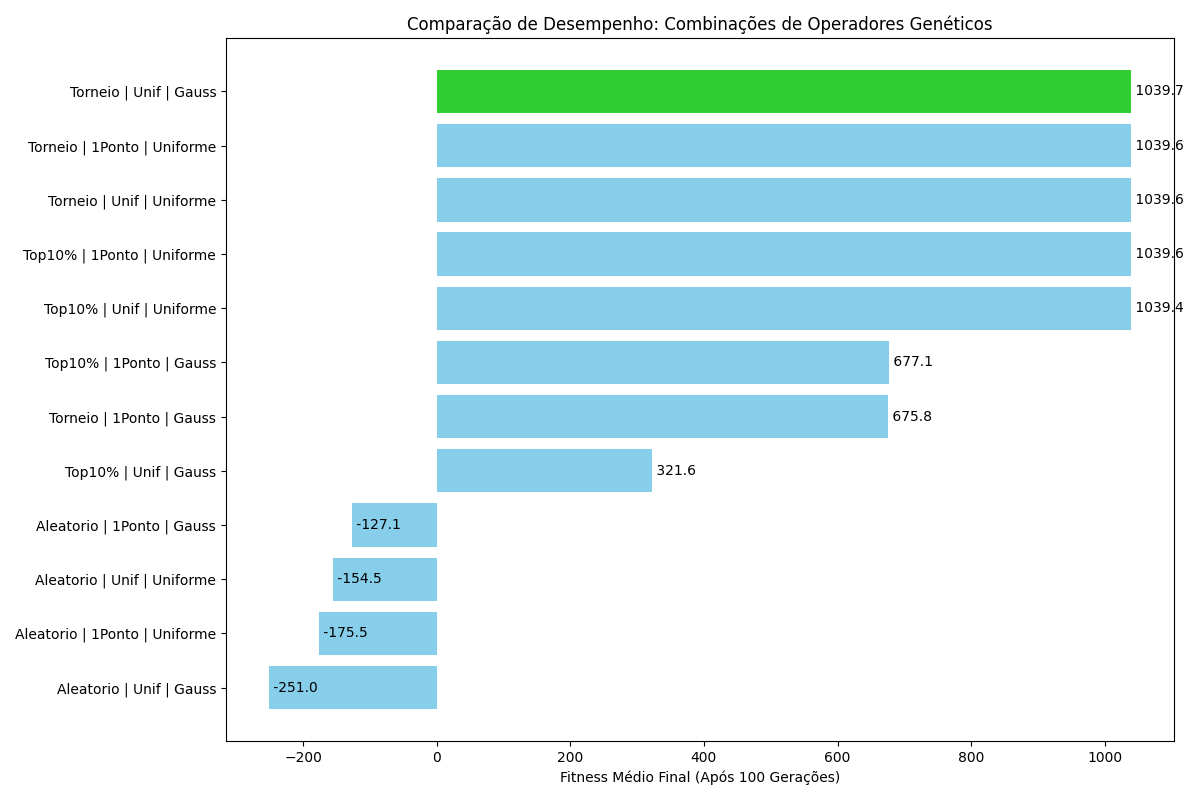
\includegraphics[width=0.9\textwidth]{comparacao_operadores.png}
    \caption{Comparação empírica de diferentes combinações de operadores genéticos.}
    \label{fig:operadores}
\end{figure}

\section{Meta 1: Aterragem em Ambiente Estático}
Na Meta 1, o vento está desligado (\texttt{ENABLE\_WIND = False}). O objetivo é afinar os parâmetros de evolução e formular uma função objetivo (fitness) contínua que guie a nave até à plataforma.

\subsection{Função Objetivo Original}
A função inicial fornecida avaliava de forma "esparsa" apenas o ponto de impacto, o que levava a comportamentos indesejados. Desenvolvemos uma função melhorada que avalia o estado final da simulação considerando:
\begin{enumerate}
    \item \textbf{Distância e Velocidade:} Penalizações baseadas na distância Euclidiana ao centro e na velocidade do impacto, ensinando a nave a travar.
    \item \textbf{Estabilidade:} Penalizações pela inclinação e velocidade angular.
    \item \textbf{Recompensa de Aterragem:} Um bónus massivo (+1000 pontos) caso a nave pouse de forma perfeita.
\end{enumerate}

\subsection{Estudo Paramétrico e Resultados (Tabela 2)}
Para encontrar a configuração ideal, realizámos as 8 experiências obrigatórias, repetindo cada uma 5 vezes para garantir significado estatístico. Avaliámos também o impacto do tamanho da população (Figura \ref{fig:populacao}). A Curva de Cotovelo revela que a partir dos 100 indivíduos os ganhos de fitness são residuais, estabelecendo $N=100$ como o compromisso ideal entre performance e custo computacional.

\begin{figure}[H]
    \centering
    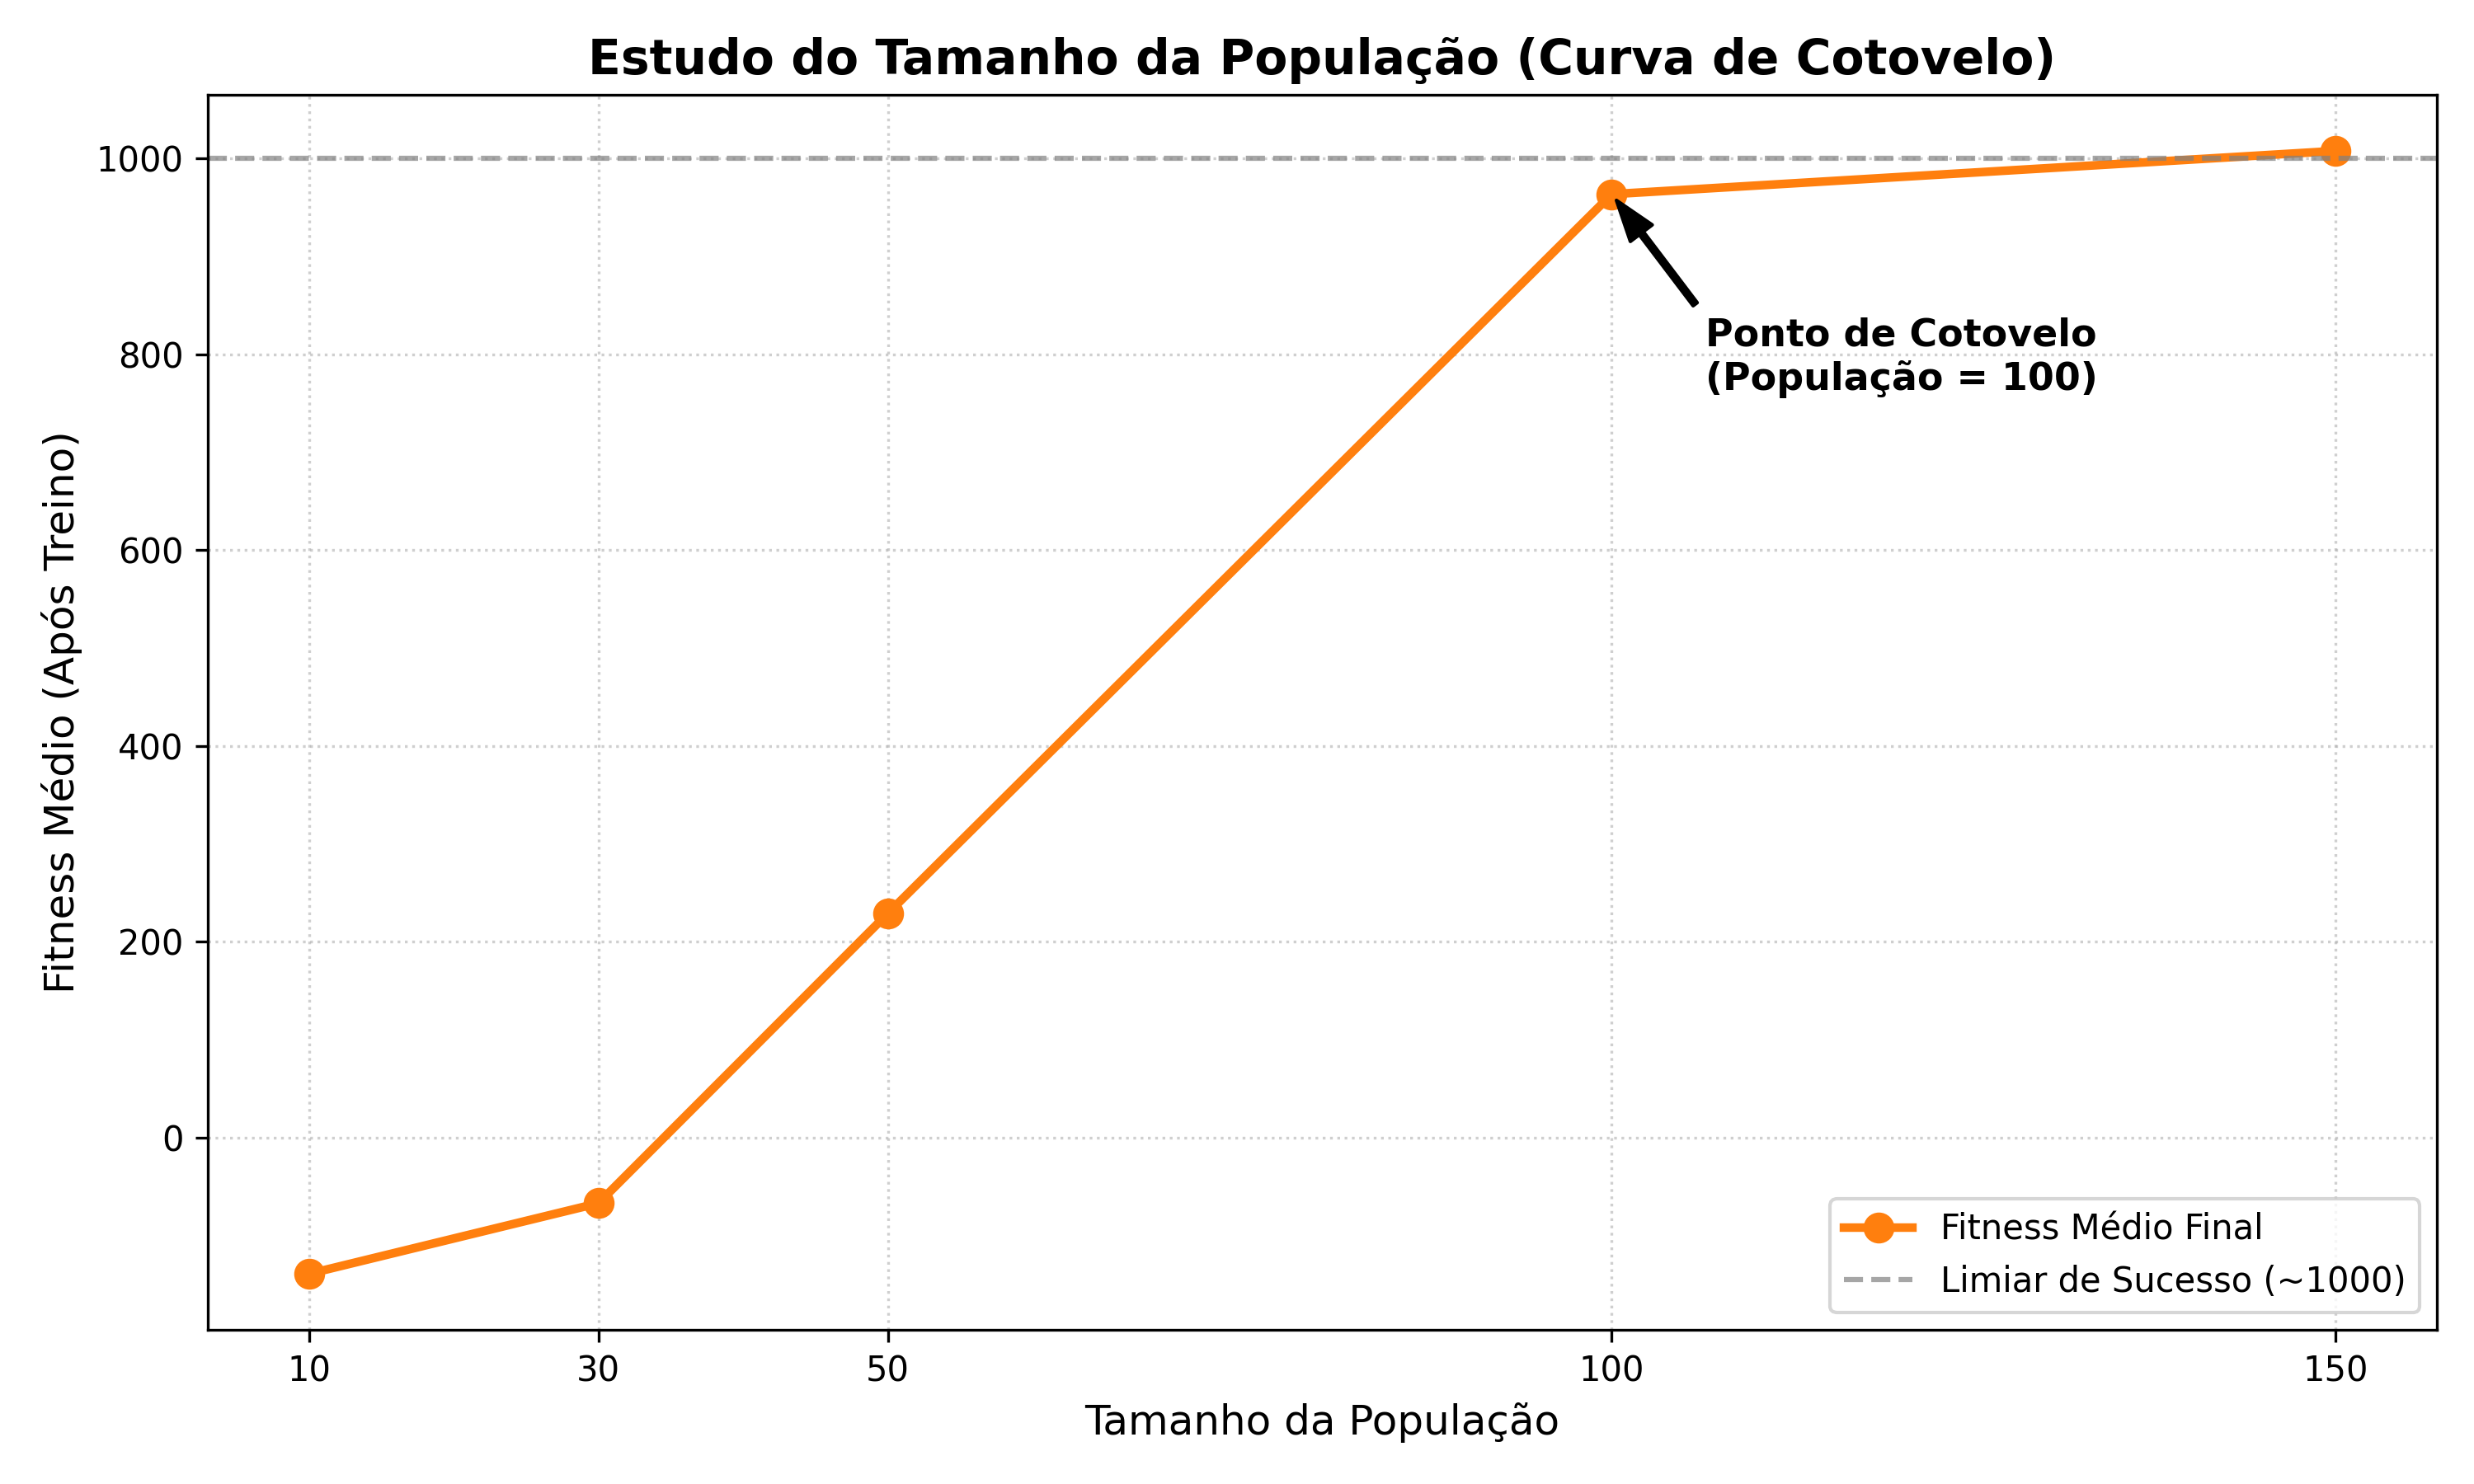
\includegraphics[width=0.7\textwidth]{estudo_populacao_real.png}
    \caption{Curva de Cotovelo para o Estudo do Tamanho da População.}
    \label{fig:populacao}
\end{figure}

Os resultados das experiências da Tabela 2 (Figura \ref{fig:tabela2}) demonstraram claramente que:
1. Um \textbf{Crossover Elevado (0.9)} é vital (Experiências 3 e 4).
2. O \textbf{Elitismo (tamanho 1)} reduziu a diversidade genética e encravou a população, piorando os resultados nas experiências 5 a 8.
3. \textbf{A Experiência 3} (Mutação=0.008, Crossover=0.9, Elite=0) obteve uma taxa de sucesso esmagadora de \textbf{97.0\%} e o menor desvio padrão ($\pm$ 1.79\%).

\begin{figure}[H]
    \centering
    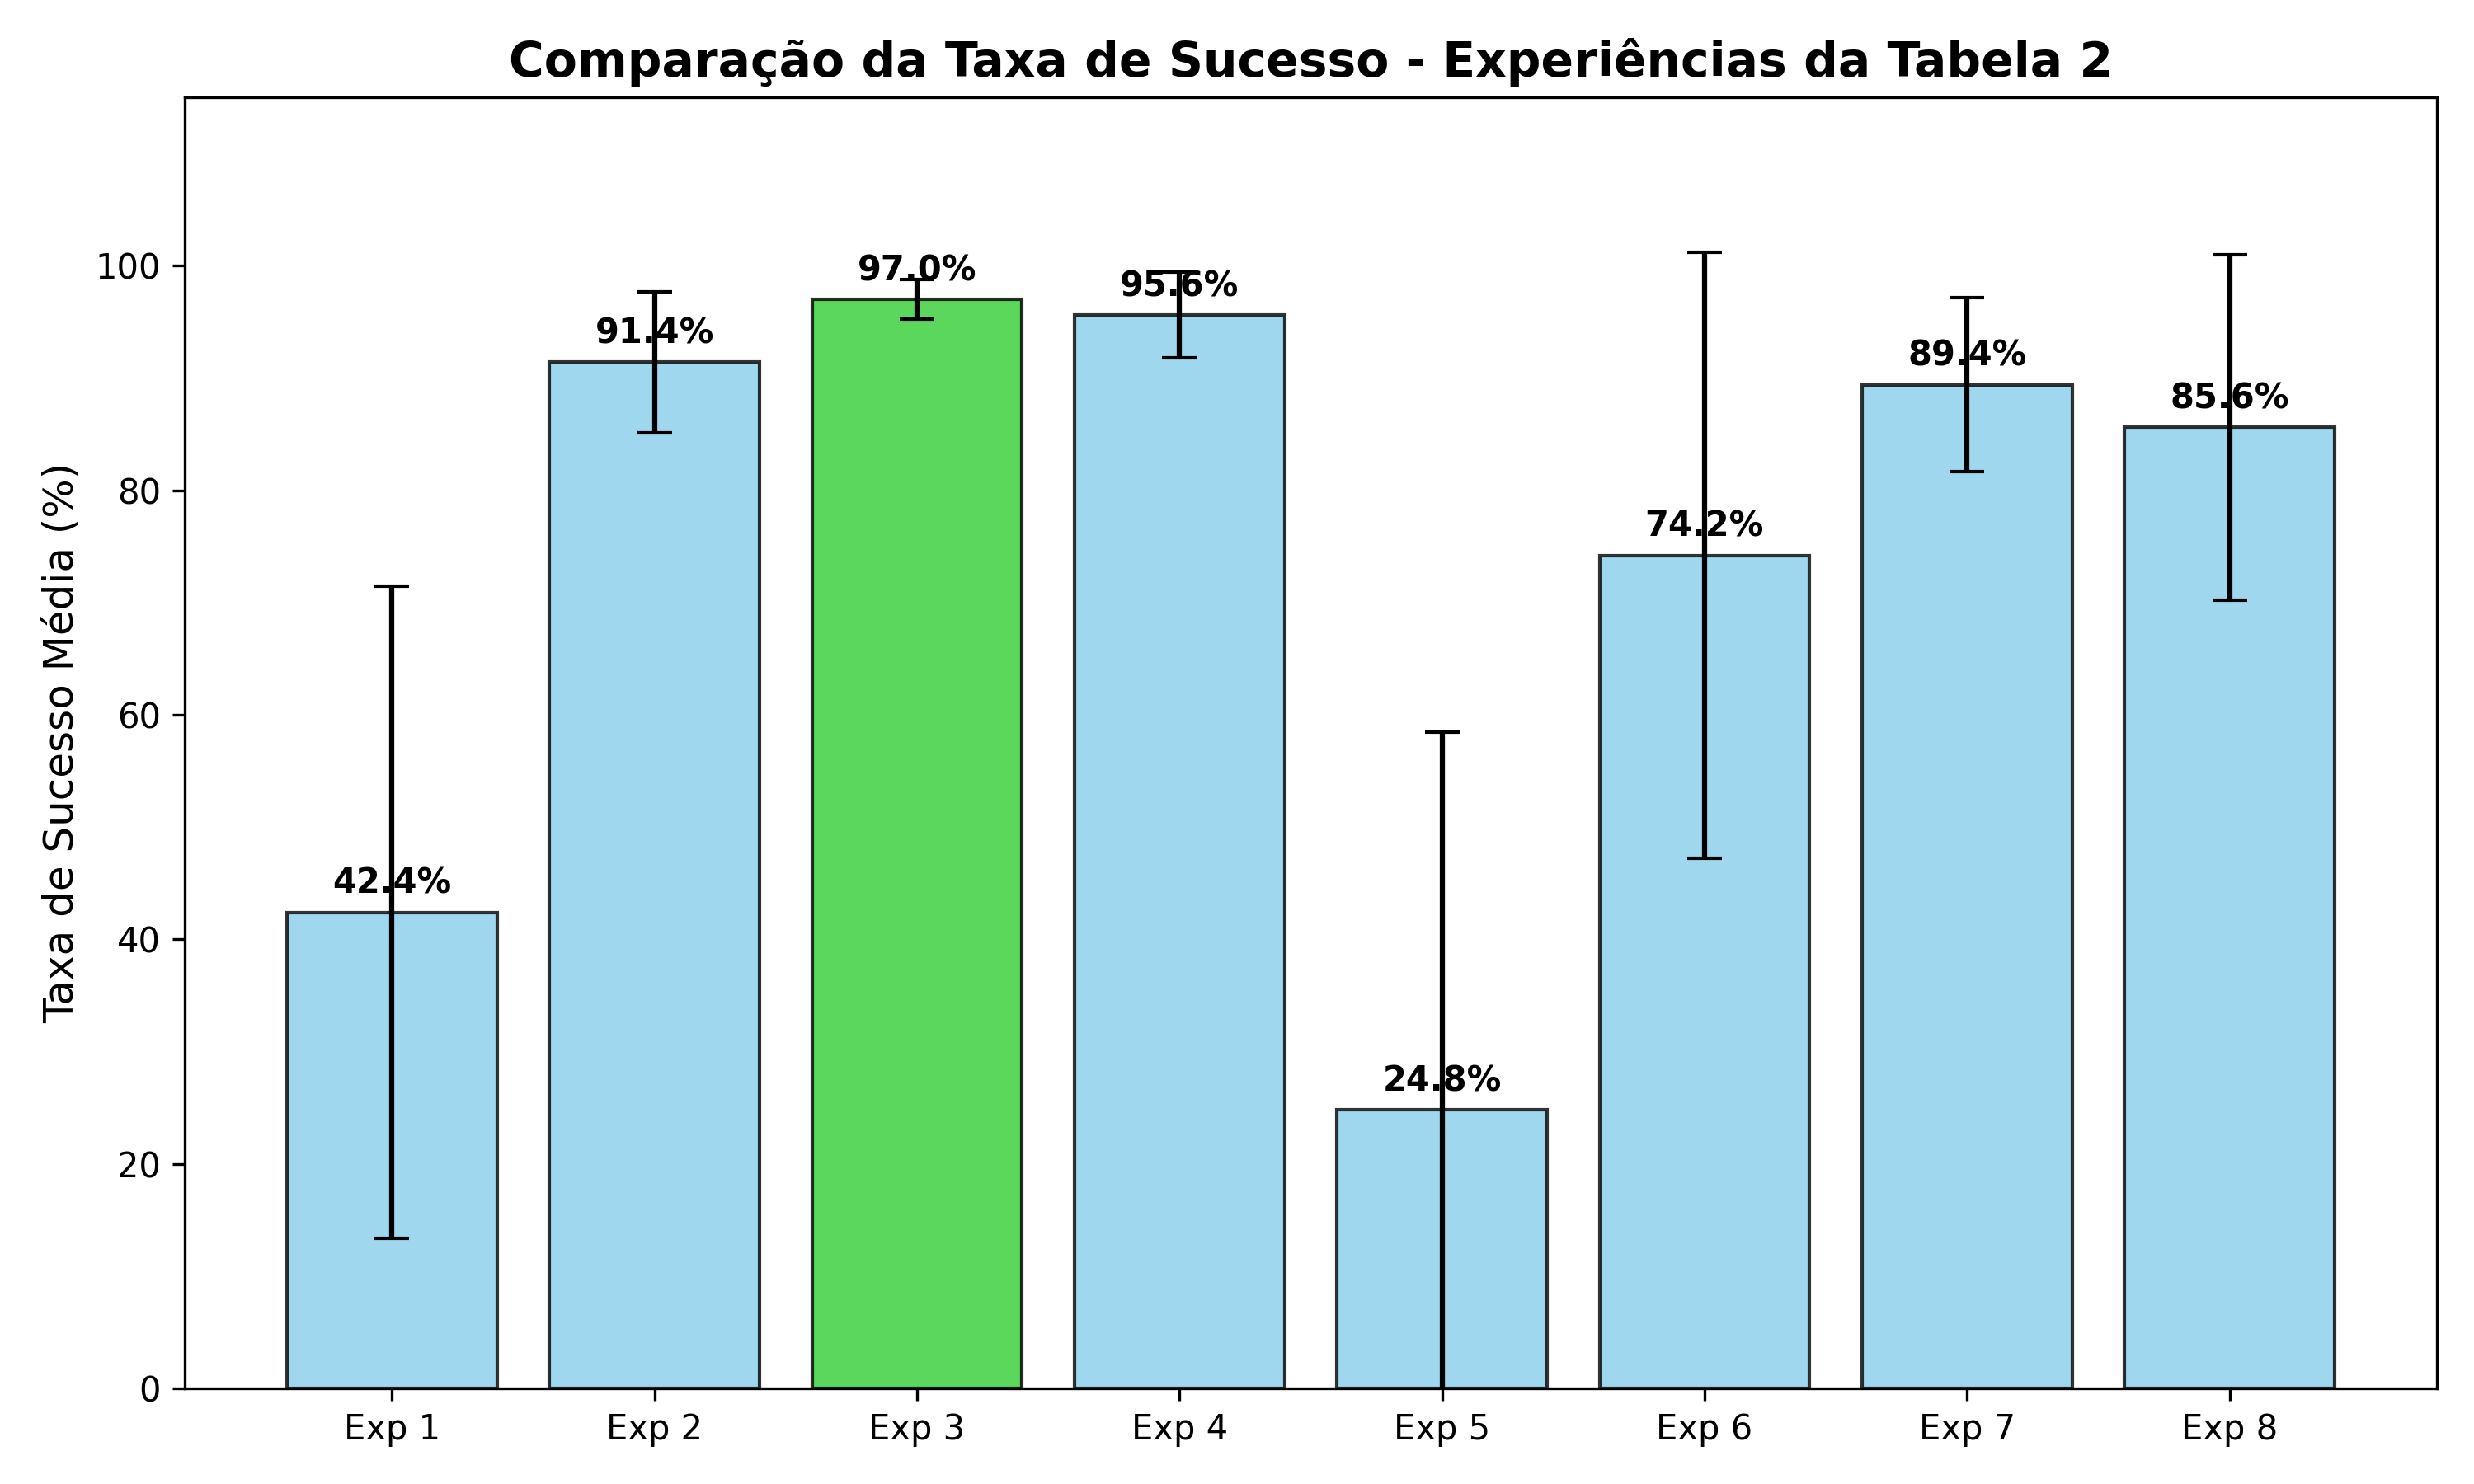
\includegraphics[width=0.85\textwidth]{grafico_taxa_sucesso.png}
    \caption{Taxa de Sucesso Média nas 8 experiências.}
    \label{fig:tabela2}
\end{figure}

A Figura \ref{fig:curva_meta1} demonstra a curva de aprendizagem da nossa melhor execução. O fitness sobre rapidamente nas primeiras 20 gerações (fase de exploração) e estabiliza acima da linha de sucesso de forma perfeitamente assintótica.

\begin{figure}[H]
    \centering
    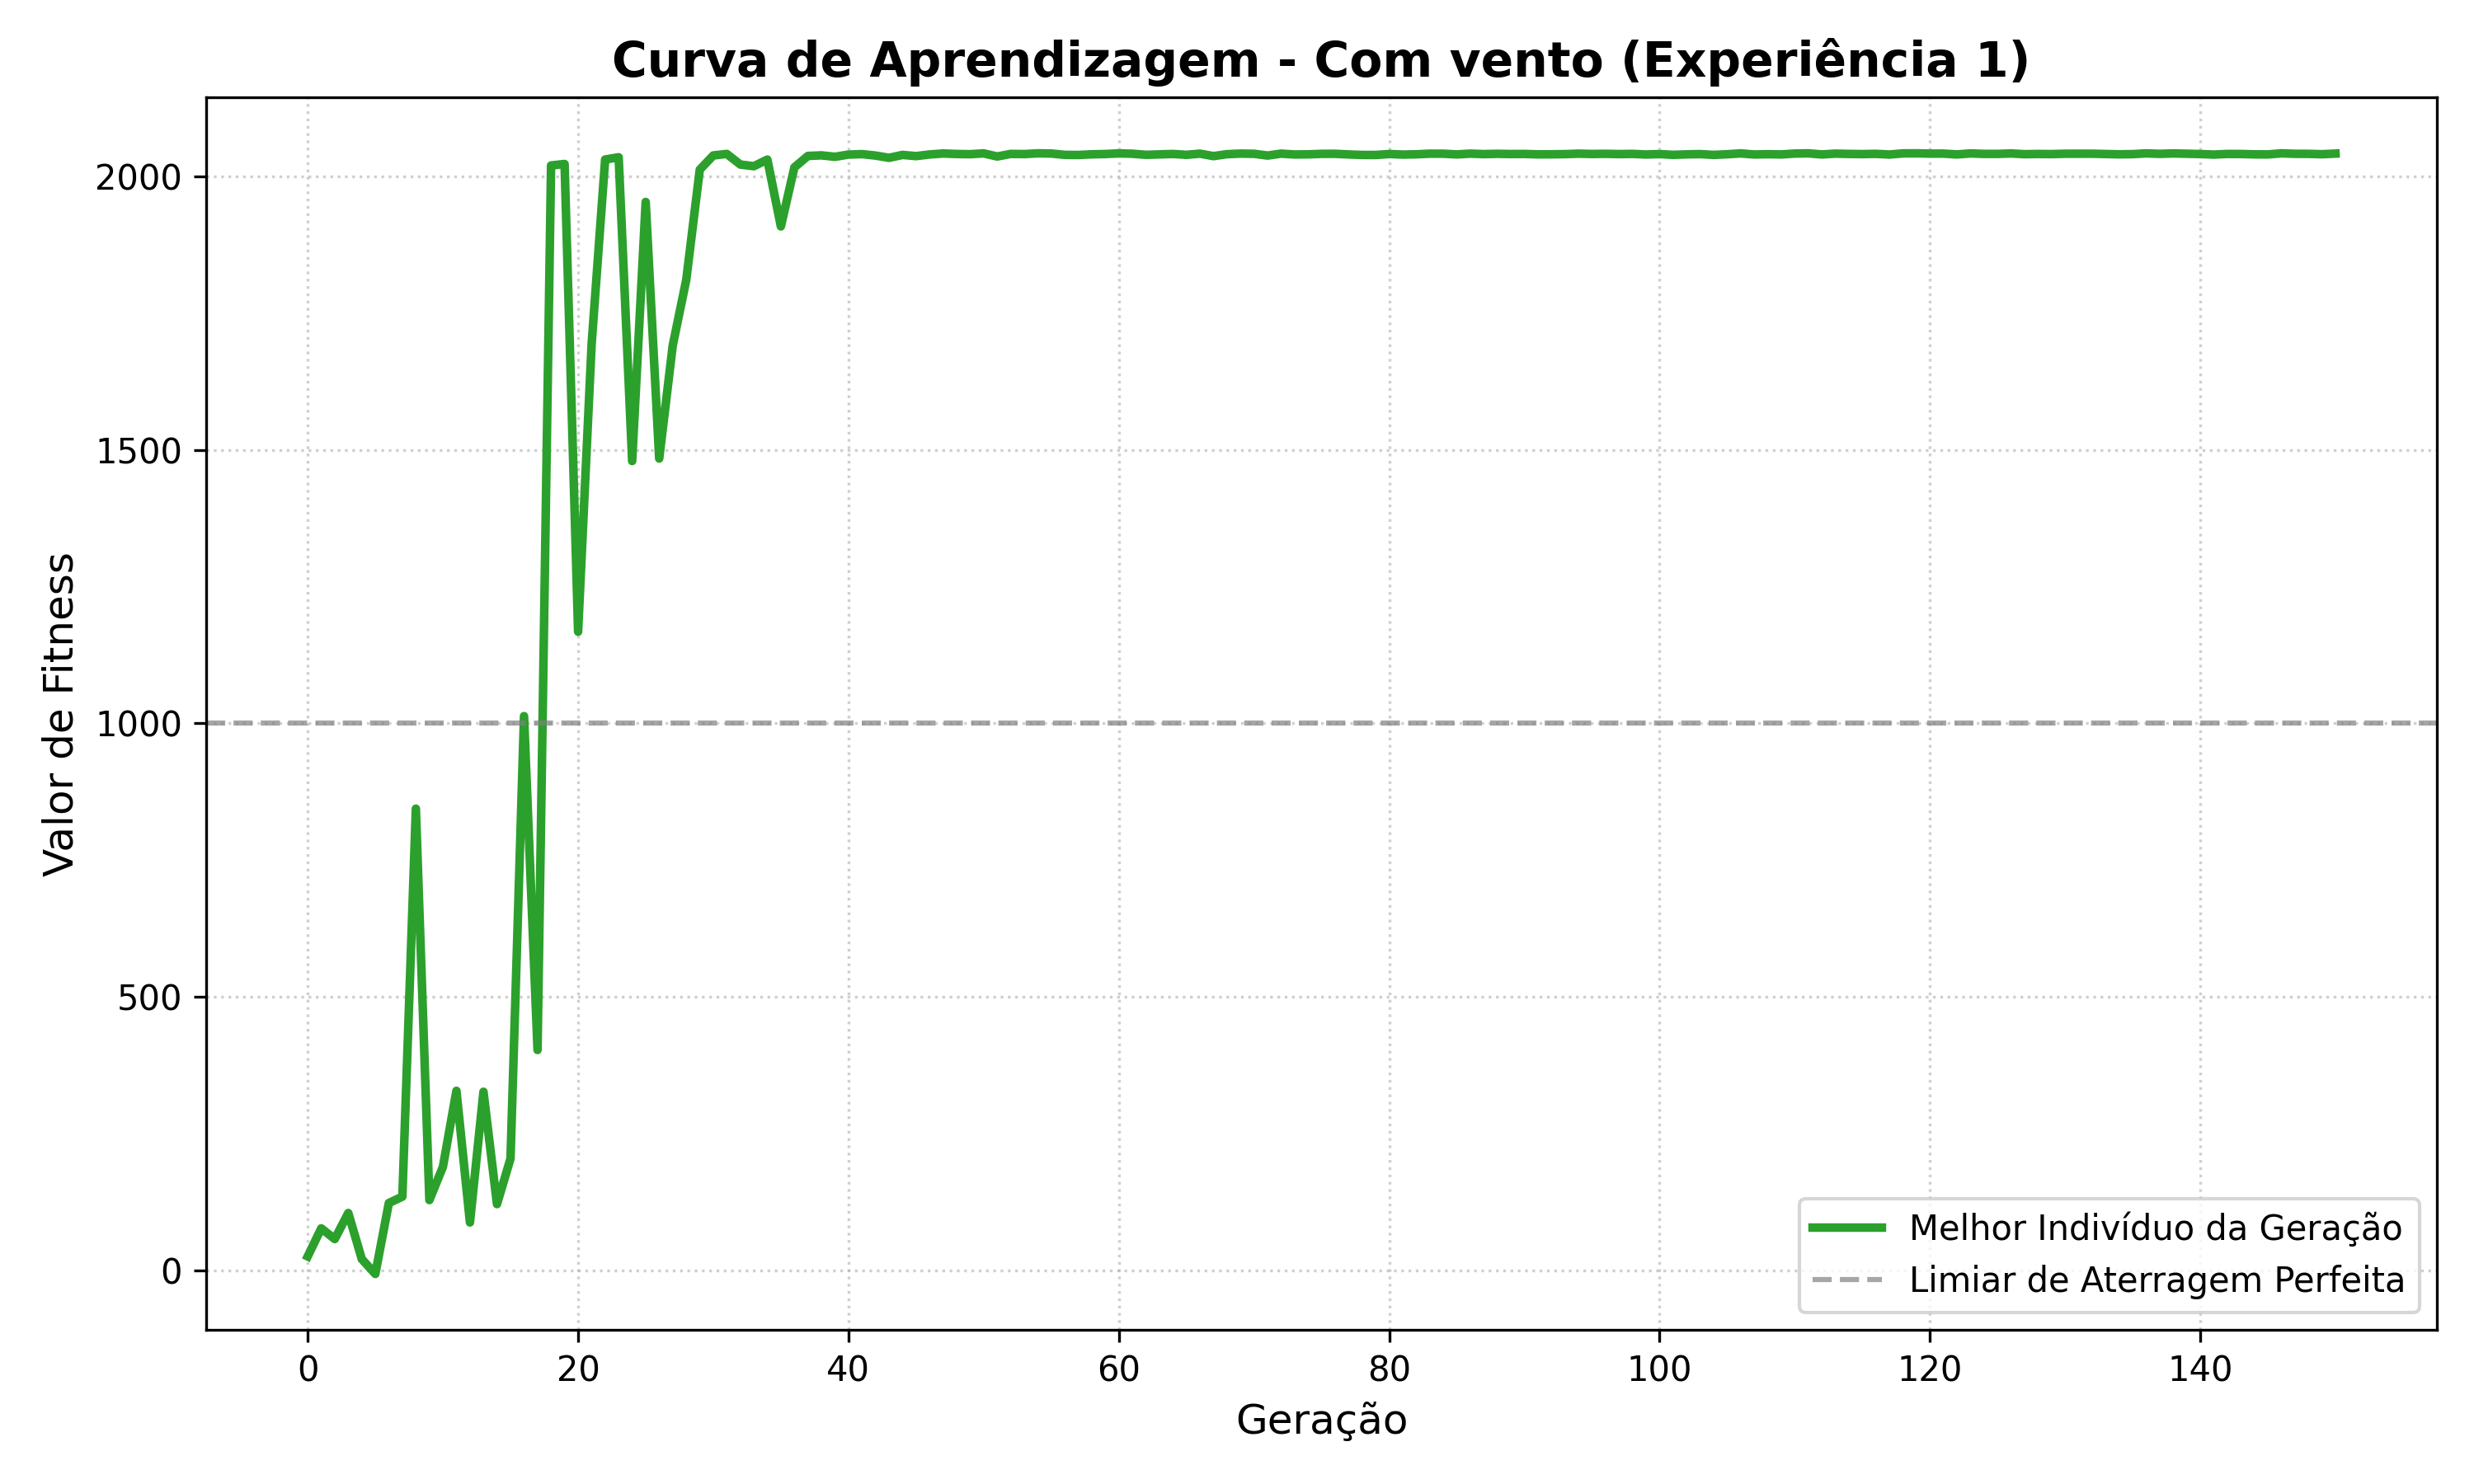
\includegraphics[width=0.8\textwidth]{curva_aprendizagem.png}
    \caption{Curva de Aprendizagem do agente ótimo na Meta 1.}
    \label{fig:curva_meta1}
\end{figure}

\section{Meta 2: O Desafio do Vento}
Ao ativarmos o vento (\texttt{WIND\_POWER = 15.0}), o ambiente tornou-se altamente estocástico.

\subsection{A Baseline e o Falso Ótimo (Suicídio)}
Submetemos o nosso agente "campeão" da Meta 1 ao vento, mantendo a função objetivo focada apenas no estado final. O resultado foi uma queda catastrófica na taxa de sucesso para \textbf{19.8\%}. Constatámos a ocorrência de \textit{Overfitting} ao ruído: os agentes decoravam uma trajetória para uma rajada de vento específica, falhando perante as variações dos testes finais (Figura \ref{fig:impacto_vento}).

\begin{figure}[H]
    \centering
    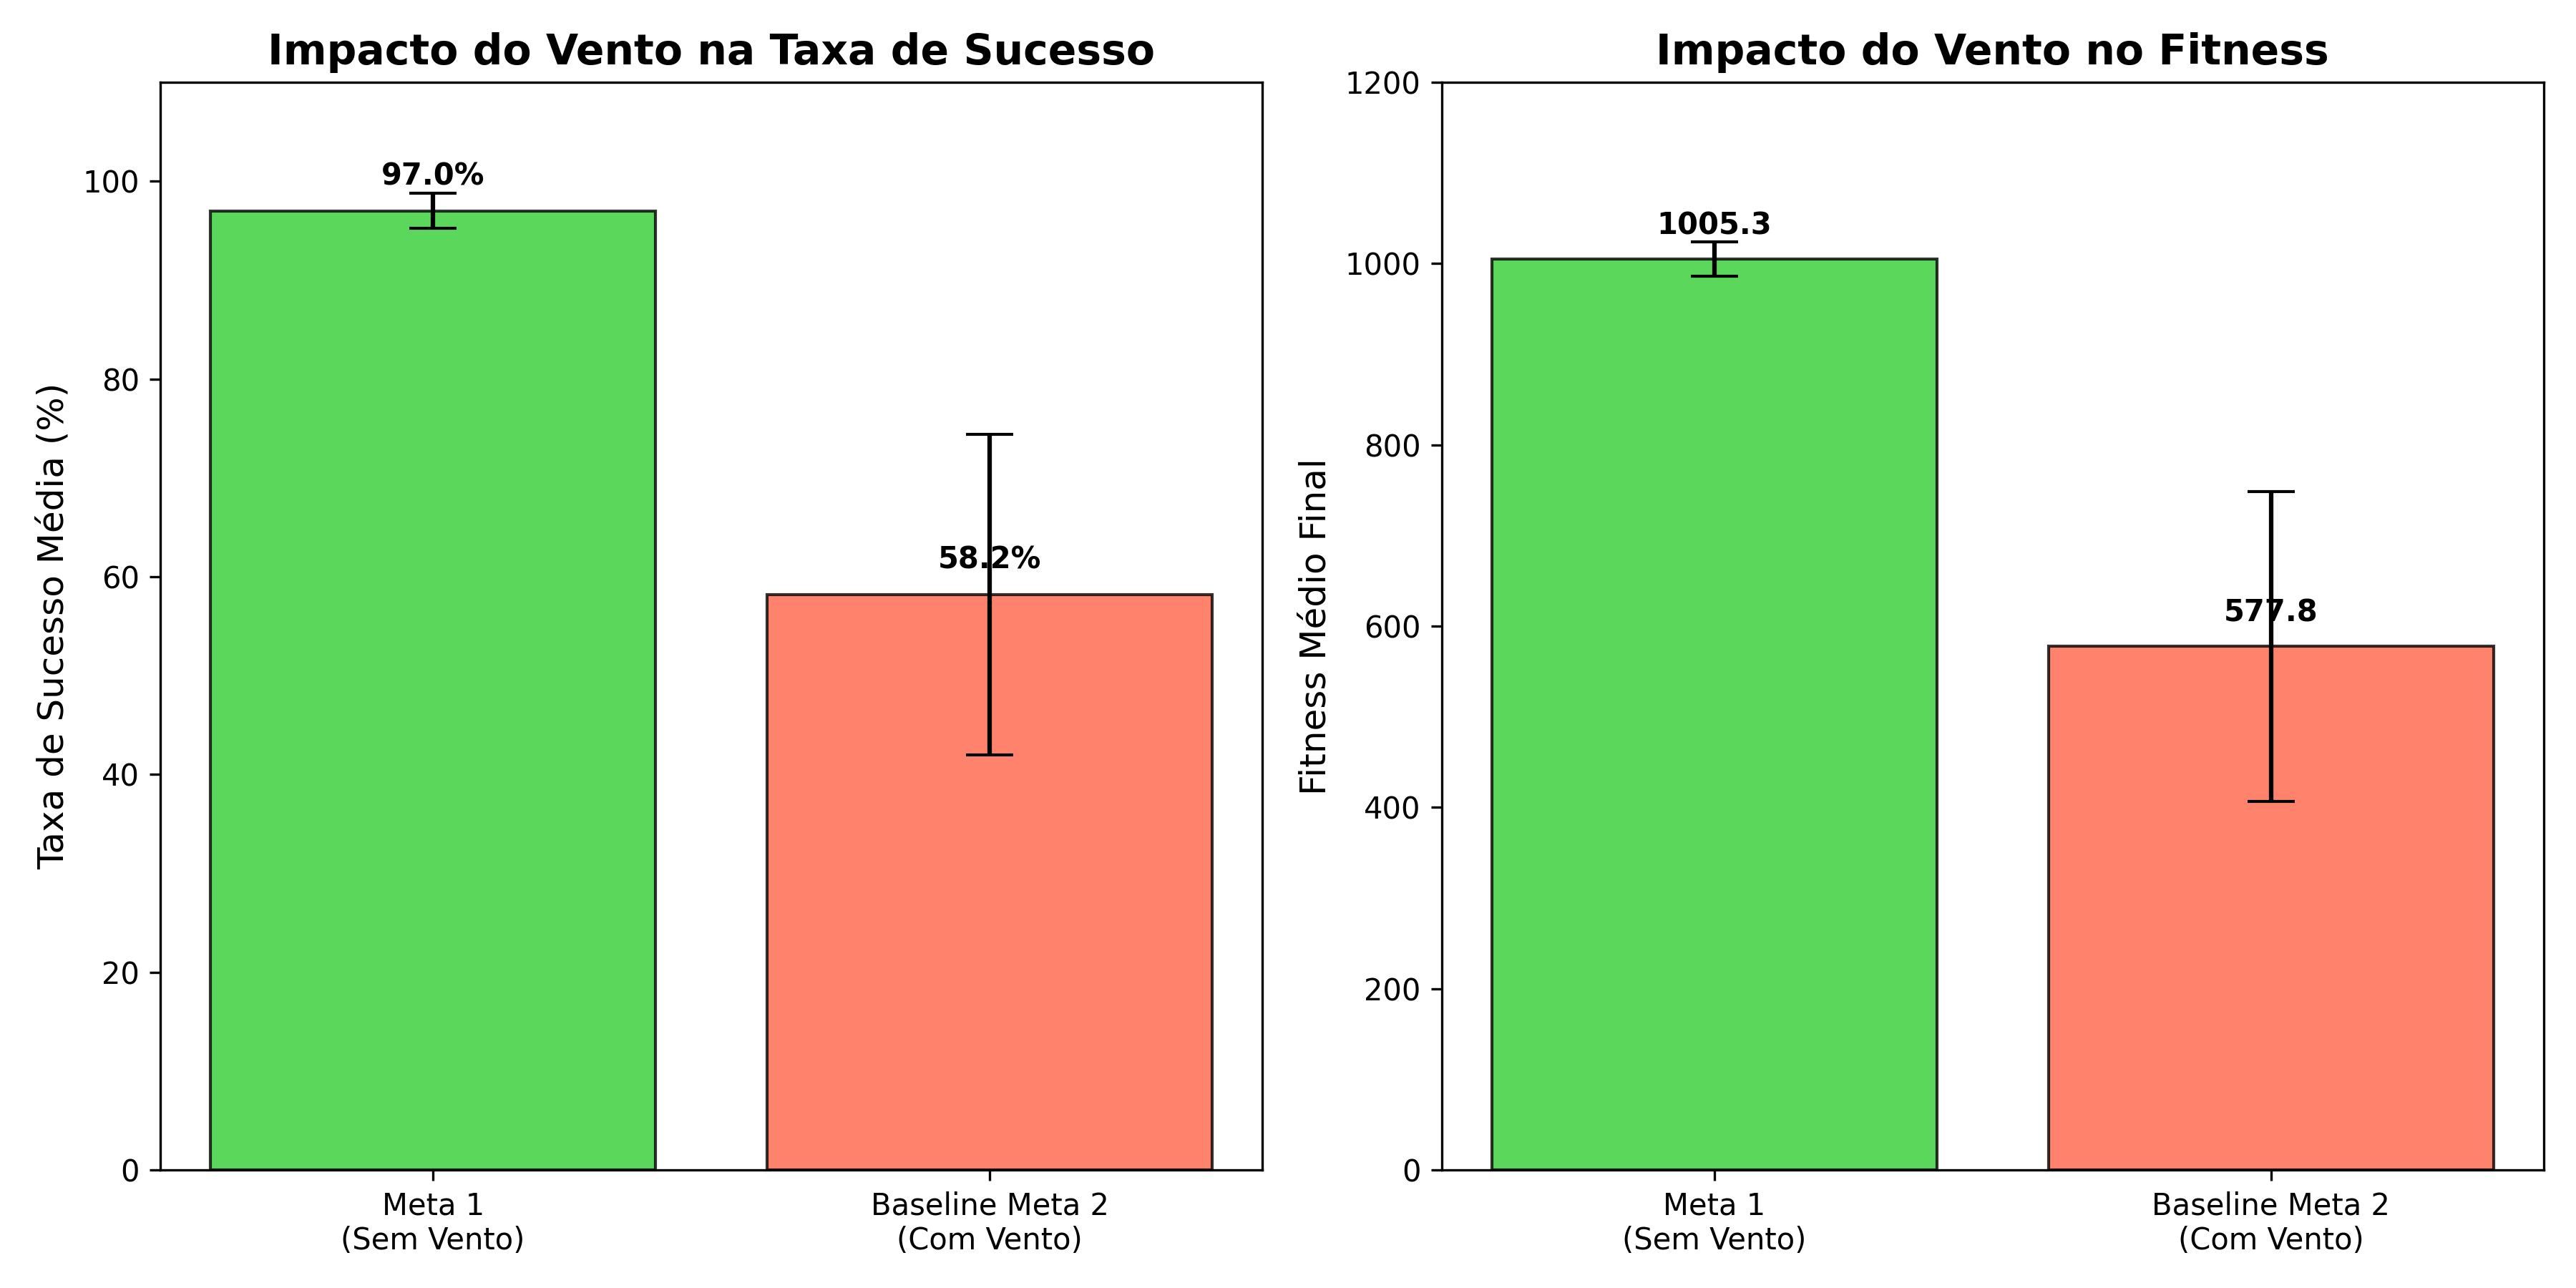
\includegraphics[width=0.8\textwidth]{impacto_vento.png}
    \caption{A queda de performance do agente perante o ambiente estocástico.}
    \label{fig:impacto_vento}
\end{figure}

Numa primeira tentativa de correção, penalizámos a distância horizontal \textit{a cada frame} da simulação. O algoritmo explorou esta matemática cometendo \textbf{"suicídio"}: a rede neuronal percebeu que despenhar a nave no step 50 resultava em menos penalizações acumuladas do que tentar voar até ao step 500.

\subsection{A Solução: Reward Shaping (O Corredor Central)}
Sendo imperativo avaliar a capacidade de lutar contra o vento (sem alterar a função que efetua a simulação ou faz médias em treino), redesenhámos completamente a função objetivo. A nossa abordagem final estabelece um \textbf{Corredor Central}:
\begin{itemize}
    \item \textbf{Penalizações Pesadas no Fim:} Multiplicámos a penalização por impacto violento para desencorajar o falso ótimo de suicídio.
    \item \textbf{Recompensa de Estabilidade:} Iteramos sobre toda a simulação e damos uma recompensa positiva (+2.0) a cada frame em que o agente se encontra no centro (\texttt{abs(x) < 0.3}), penalizando-o (-1.0) se sair da rota.
    \item \textbf{Recompensa de Ouro:} O bónus de aterragem subiu para 3000, garantindo que "sobreviver no centro" nunca superaria "aterrar no centro".
\end{itemize}

\subsection{Resultados Finais}
A implementação desta hierarquia de pontuação cortou o espaço de manobra do algoritmo para "hacks". Reativámos as 150 gerações para acomodar a complexidade de aprendizagem. Como evidencia a Figura \ref{fig:meta2_comparacao}, atingimos uma taxa de sucesso média de \textbf{64.2\%}, superando largamente a \textit{baseline} (Função Antiga).

\begin{figure}[H]
    \centering
    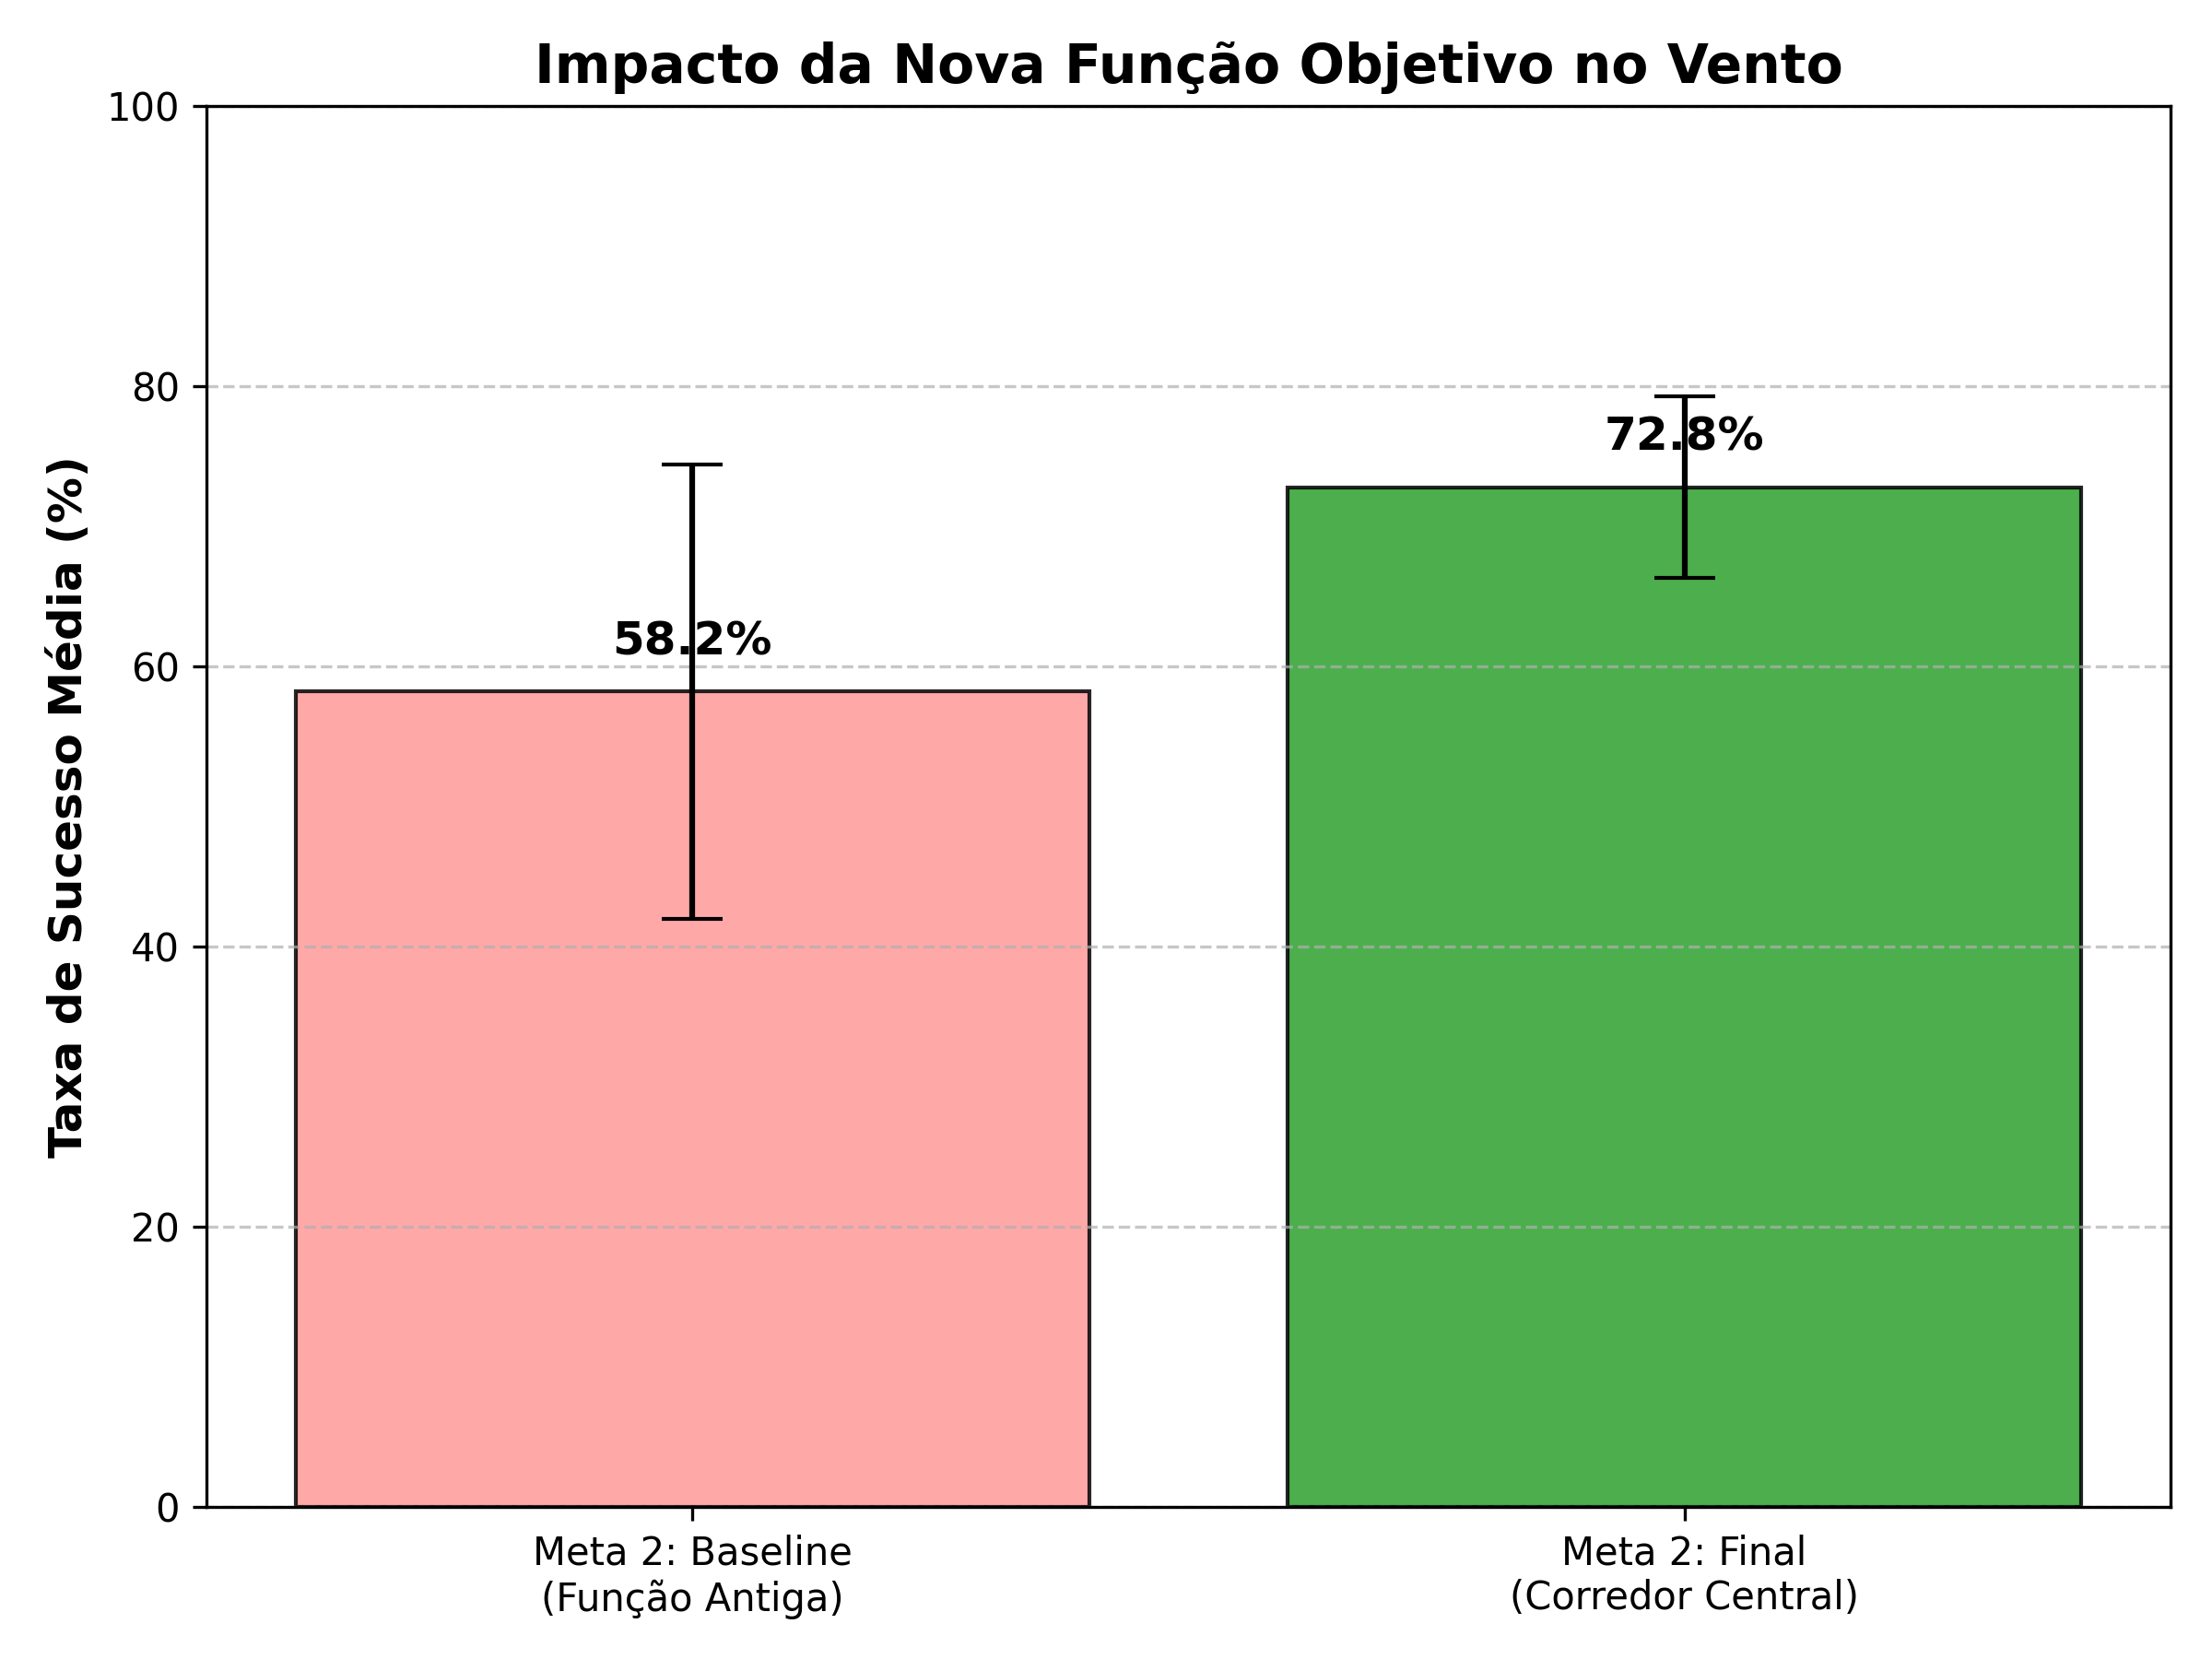
\includegraphics[width=0.8\textwidth]{meta2_comparacao.png}
    \caption{Comparação da Taxa de Sucesso Média (Nova vs Antiga Função Objetivo).}
    \label{fig:meta2_comparacao}
\end{figure}

Ao analisar as 5 execuções independentes (Figura \ref{fig:meta2_runs}), notamos que o algoritmo é muito consistente: 4 em 5 execuções convergiram para soluções robustas (entre 66\% e 74\% de sucesso) perante ventos aleatórios fortíssimos. Apenas a Run 0 ficou presa num ótimo local inferior, o que é esperado devido à estocasticidade do vento e à limitação de avaliarmos apenas 1 episódio por geração durante o treino.

\begin{figure}[H]
    \centering
    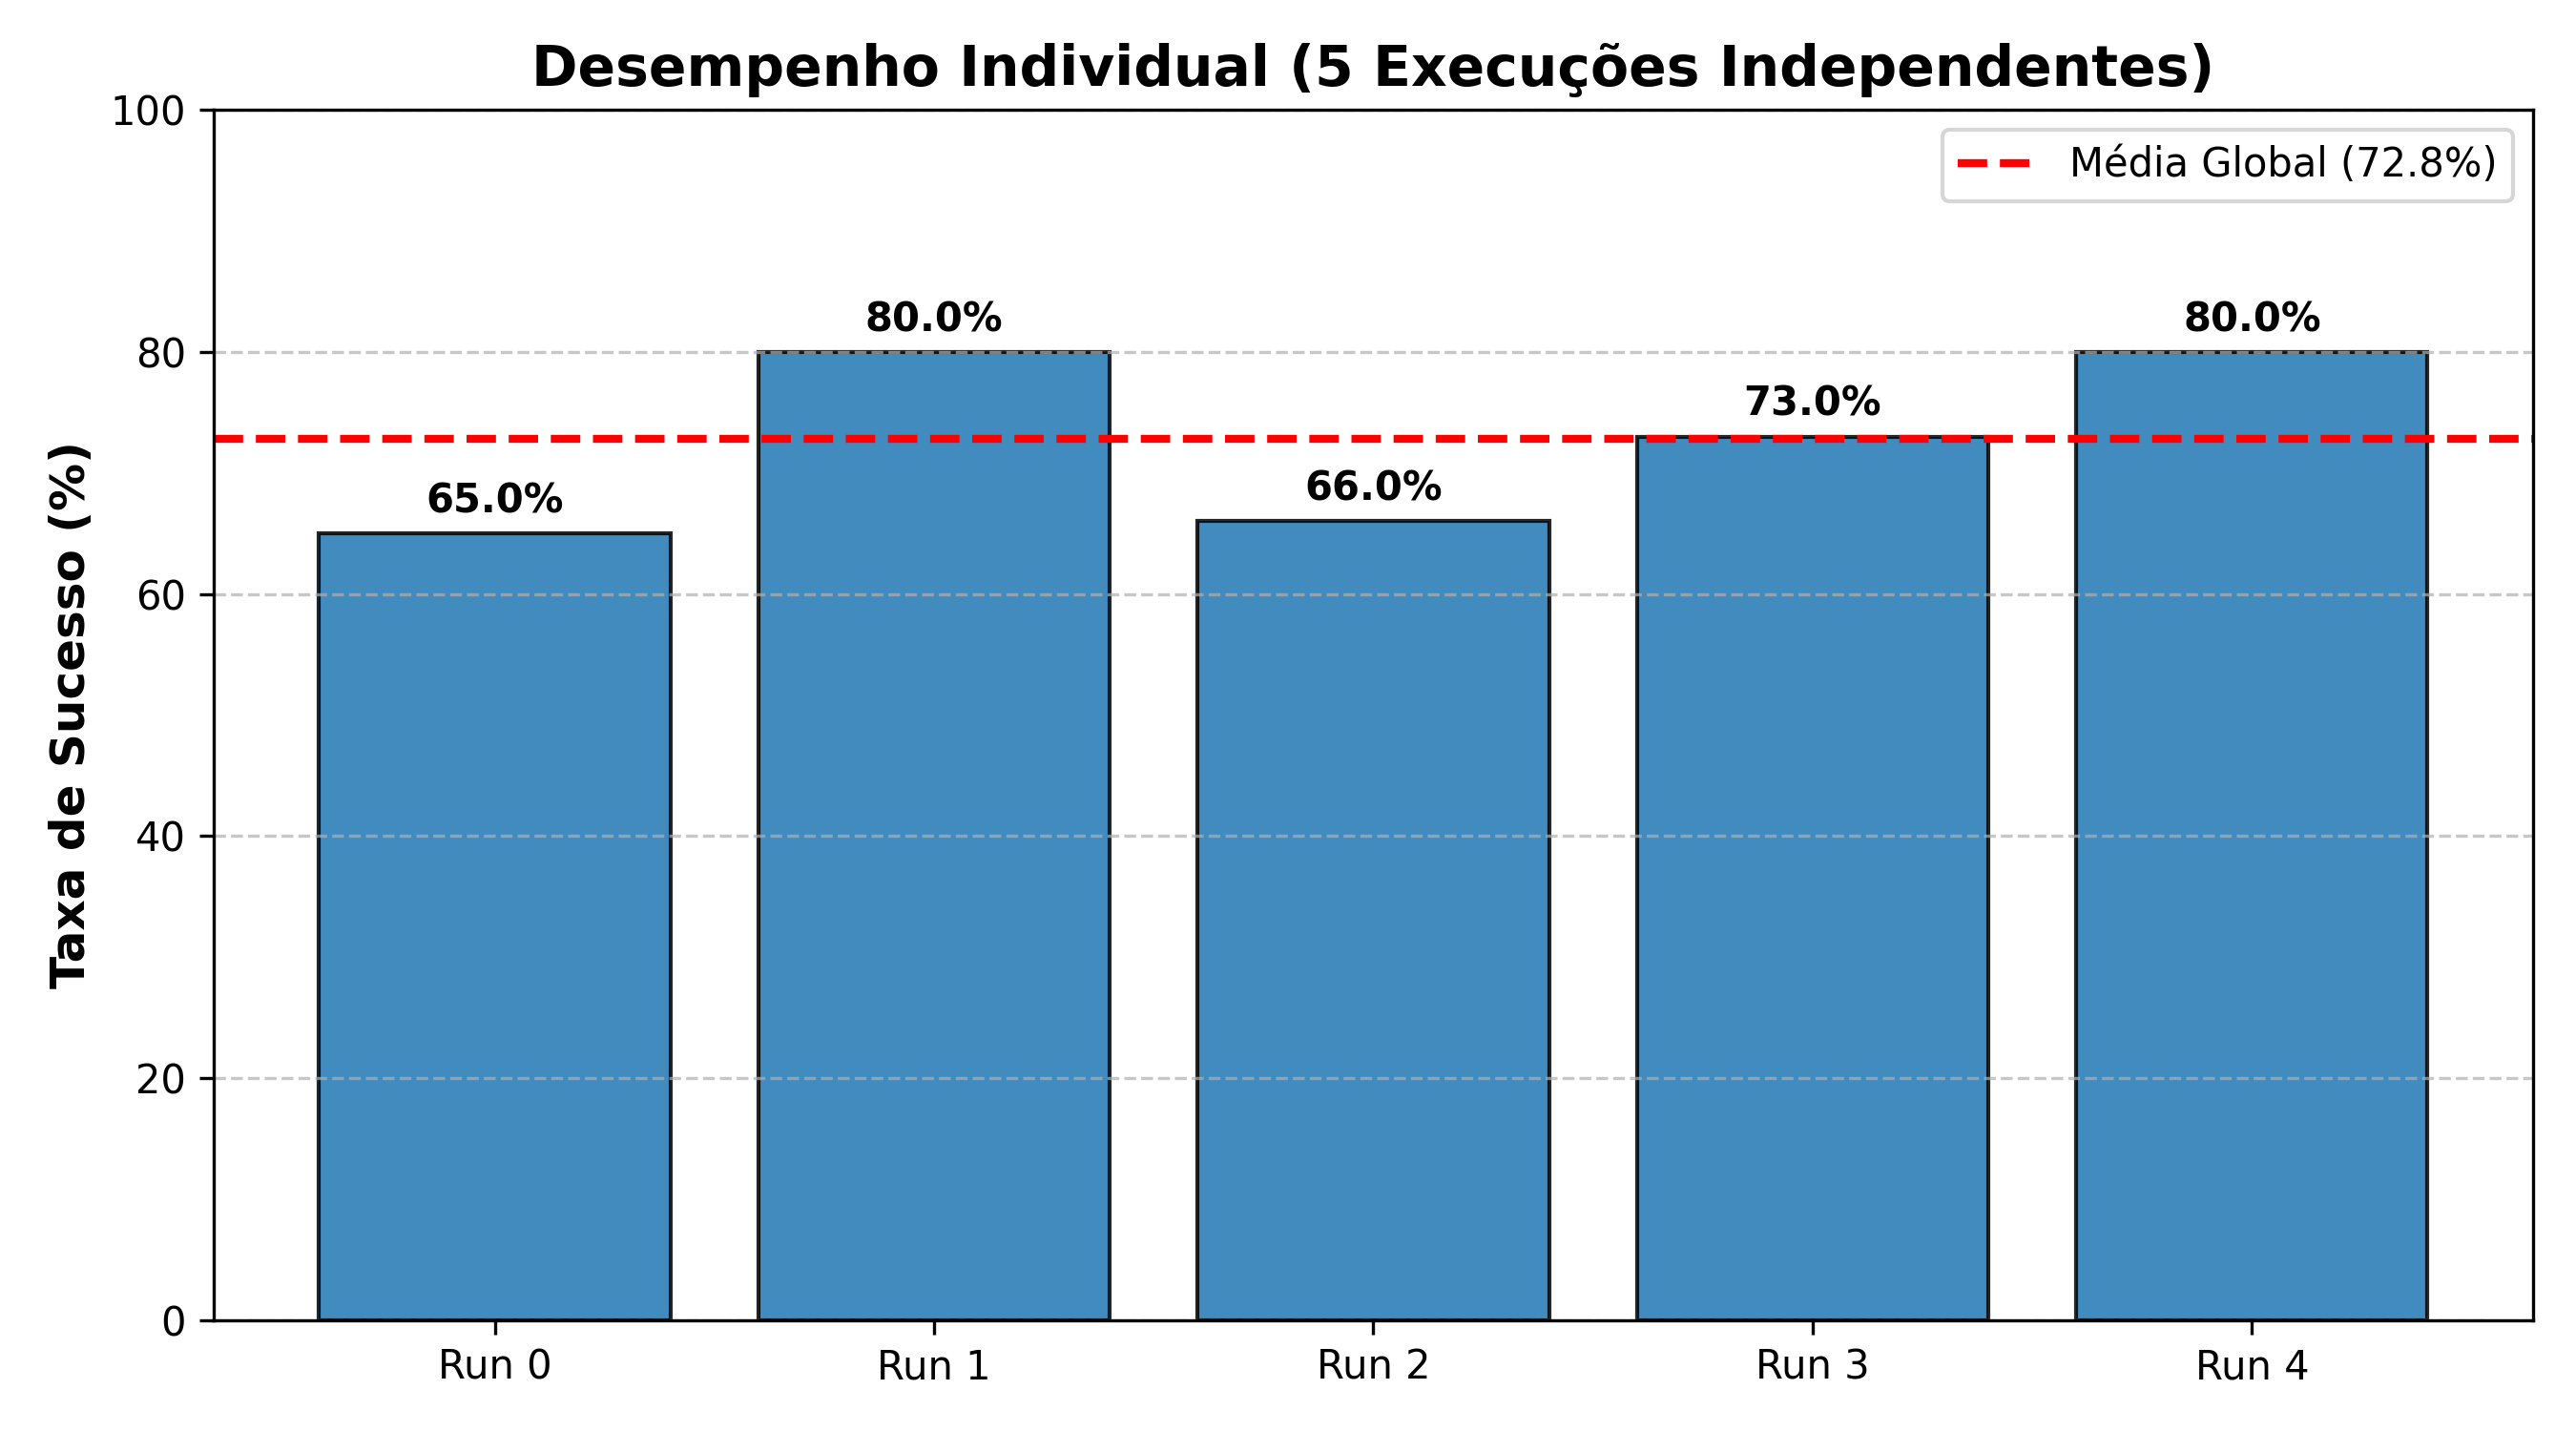
\includegraphics[width=0.8\textwidth]{meta2_runs.png}
    \caption{Consistência das 5 runs com o Reward Shaping final (Meta 2).}
    \label{fig:meta2_runs}
\end{figure}

\section{Declaração de Uso de Inteligência Artificial}
Em conformidade com o código de conduta estabelecido, declaramos que ferramentas de Inteligência Artificial (modelos baseados em LLMs, nomeadamente Gemini) foram utilizadas no decurso deste projeto com os seguintes propósitos:
\begin{itemize}
    \item Auxílio na estruturação modular do relatório em LaTeX.
    \item Escrita de \textit{scripts} em Python (matplotlib/numpy) para automatizar a leitura dos ficheiros \texttt{logX.txt} e gerar os gráficos comparativos.
    \item Brainstorming matemático para a elaboração de funções objetivo ("Reward Shaping") que prevenissem o problema dos ótimos locais sob condições de vento.
\end{itemize}
A conceção lógica do pipeline genético, a execução exaustiva das experiências, e toda a análise crítica e empírica dos resultados refletida no texto é fruto do entendimento e integração de conhecimentos dos autores, estando totalmente preparados para demonstrar domínio absoluto do código desenvolvido em contexto de defesa.

\section{Conclusão}
O presente trabalho permitiu aprofundar de forma tangível as dinâmicas de um Algoritmo Evolucionário. A transição da Meta 1 para a Meta 2 reforçou a grande lição da Inteligência Artificial: o comportamento de um agente é tão bom quanto a robustez da Função Objetivo que o avalia. Através da modelação cuidadosa de recompensas, fomos capazes de forçar o surgimento de mecanismos complexos (uso reativo de propulsores laterais) a partir de uma arquitetura simples de Neuroevolução, atingindo uma performance assinalável num ambiente severamente estocástico.

\end{document}
